\documentclass[a4paper,twocolumn]{article}


\usepackage[sc]{mathpazo} % Use the Palatino font
\usepackage[T1]{fontenc} % Use 8-bit encoding that has 256 glyphs
\usepackage[utf8]{inputenc} % Use utf-8 as encoding
\linespread{1.05} % Line spacing - Palatino needs more space between lines
\usepackage{microtype} % Slightly tweak font spacing for aesthetics

\usepackage[english]{babel} % Language hyphenation and typographical rules
%\usepackage[galician]{babel} % Change to this if using galician
%\usepackage[spanish]{babel} % Change to this if using spanish

\usepackage[hmarginratio=1:1,top=32mm,columnsep=20pt]{geometry} % Document margins
\usepackage[hang, small,labelfont=bf,up,textfont=it,up]{caption} % Custom captions under/above floats in tables or figures
\usepackage{booktabs} % Horizontal rules in tables

\usepackage{enumitem} % Customized lists
\setlist[itemize]{noitemsep} % Make itemize lists more compact

\usepackage{abstract} % Allows abstract customization
\renewcommand{\abstractnamefont}{\normalfont\bfseries} % Set the "Abstract" text to bold
\renewcommand{\abstracttextfont}{\normalfont\small\itshape} % Set the abstract itself to small italic text

\usepackage{titlesec} % Allows customization of titles
\renewcommand\thesection{\Roman{section}} % Roman numerals for the sections
\renewcommand\thesubsection{\Alph{subsection}} % roman numerals for subsections
\titleformat{\section}[block]{\large\scshape\centering}{\thesection.}{1em}{} % Change the look of the section titles
\titleformat{\subsection}[block]{\large}{\thesubsection.}{1em}{} % Change the look of the section titles

\usepackage{multirow}

\usepackage{graphicx}

\usepackage{fancyhdr} % Headers and footers
\pagestyle{fancy} % All pages have headers and footers
\fancyhead{} % Blank out the default header
\fancyfoot{} % Blank out the default footer
%\fancyhead[C]{Running title $\bullet$ May 2016 $\bullet$ Vol. XXI, No. 1} % Custom header text
\fancyfoot[C]{\thepage} % Custom footer text

\usepackage{titling} % Customizing the title section

\usepackage{hyperref} % For hyperlinks in the PDF

%----------------------------------------------------------------------------------------
%	TITLE SECTION
%----------------------------------------------------------------------------------------

\setlength{\droptitle}{-4\baselineskip} % Move the title up

\pretitle{\begin{center}\huge\bfseries} % Article title formatting
	\posttitle{\end{center}} % Article title closing formatting

\title{Report on potential GPU'S for Name}

\author{\textsc{Uxío García Andrade} \\[1ex]
	\normalsize Laboratorio de Fundamentos de Computadores I\\
	\normalsize Grupo 01 \\
	\normalsize \uxio.garcia.andrade@rai.usc.es
\date{\06/03/2018}
\renewcommand{\maketitlehookd}{

	\begin{abstract}
		\noindent Comparative analysis of Graphics Processing Units (GPUs), centered on its deep learning suitability. In order to select which GPU best fits the needs of the company, several cutting edge technologies are subjected to analysis, taking into consideration features such as price, memory bandwith, processing power or VRAM size. Furthermore, GPUs' performance is tested and contrasted by the results of diverse benchmark, as well as other prestigious studies to back up our conclusions.\\\mbox{}\\
		 \textbf{\textit{Keywords}: GPU, deep learning, machine learning, AI, NVIDIA, Benchmark}
	\end{abstract}
}

%----------------------------------------------------------------------------------------

\begin{document}

	% Print the title
\maketitle
%
	%----------------------------------------------------------------------------------------
	%	ARTICLE CONTENTS
	%----------------------------------------------------------------------------------------

	\section{Introduction}

	Machine Learning is the field of study that gives computers the ability to learn without being explicitly programmed~\cite{andrewNG}. One of its most revolutionary subfields is Deep Learning, which is based on learning data representations, as opposed to task-specific algorithms. ~\cite{wikipedia} It has countless applications, being healthcare institutions and self-driving cars companies our best clients.
	Nevertheless, the implementation of such disruptive technologies often involves expensive hardware updates. Due to this, our engineering team has been lately complaining about the lack of deep learning-oriented equipment, focusing on the paramount urge of acquiring new cost-efficient GPUs. This paper is based on the market analysis developed by ... and .

	To avoid possible merging  problems, we have decided to primarily evaluate NVIDIA GPUs, as AMD's OpenCL toolkit has some compatibility issues with major DL frameworks. This will be our most restrictive but necessary constraint.

	The rest of this paper is organized as follows. Section 2 discusses how to escrutine GPUs' suitability for DL, section 3 shows the results we have obtained, and section 4 offers conclusions.

	%------------------------------------------------

	\section{Apartado 2}

	Our research has shown that there are 3 main specifications to focus on when it comes to Deep Learning: memory bandwith, which is probably the most important one, as it determines the amount of data the GPU is able to handle; processing power, which indicates how fast the GPU can manage data; and VRAM size, although its relevance depends on the kind of work we need to do. Moreover, price and cost-efficiency will also be evaluated, as our budget restrictions play a decisive role when selecting GPUs.
	In order to compare GPUs, we have gathered information from diverse benchmarks. The first one ~\cite{directCompute} considers computational power of the GPUs, by performing general purpose computing, and taking advantage of the huge paralell computation capacity of GPUs. On the other hand, the second one ~\cite{pricePerformance} analyses performance per dollar, as we are expected to select affordable GPUs.



%\begin{table}[tb]
	%{\footnotesize
	%\caption{Valoración de especificaciones técnicas}
	%\label{tab:valora}
	%\centering
	%\begin{tabular}{|c|c|c|c|c|c|c|}
		%\hline\hline
%\textbf{TR} & \textbf{INT} & \textbf{ESC} & \textbf{DIS} & \textbf{FIA} & \textbf{TF} & \textbf{MAN} \\\hline
%5 & 10 & 9 & 7 & 7 & 8 & 3 \\\hline\hline
%\textbf{COM} & \textbf{SEG} & \textbf{COS} & \textbf{TAM} & \textbf{CON} & \textbf{Treal} & \textbf{IS} \\\hline
%1 & 6 & 5 & 10 & 10 & 2 & 6\\\hline
	%\end{tabular}
	%}
%\end{table}



%------------------------------------------------

\section{Resultados}

	Once applied an initial filter to the NVIDIA GPUs, we decided to focus on the following ones:
	\begin{itemize}
		\item GeForce GTX 1070
		\item GeForce GTX 1070 Ti
		\item GeForce GTX 1060
		\item Quadro P2000


		\begin{table}[htbp]
			\begin{center}
			\begin{tabular}{|l|l|}
				\hline
				a &	GeForce GTX 1070 & GeForce GTX 1070 Ti & GeForce GTX 1060 & Quadro P2000 \\ \hline
			Price(dinero) 10 & 20 & 30 & 40\\ \hline
			Bandwidth(GB/s) & 256 & 256 & 192 & 140 \\ \hline
			VRAM(GB) & 8 & 8 & 6 & 5\\ \hline
			CUDA Cores & 2432 & 1920 & 1280 & 1024
			\end{tabular}
			\caption{Tabla muy sencilla.}
			\label{tabla:sencilla}
			\end{center}
			\end{table}


\subsection{Benchmarks}

\begin{figure}[H]
\centering
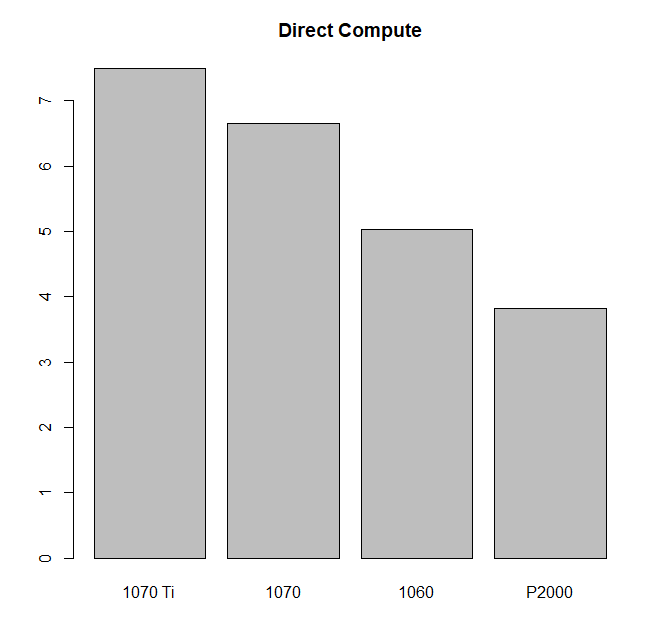
\includegraphics[width=1\textwidth]{bench1}
\end{figure}



Se presentan resultados en tablas o en figuras de modo que todas las tablas y figuras tengan un formato similar. Si son datos que nosotros no hemos obtenido, sino que son sacados de libros, artículos o webs debemos indicar la fuente de que fueron obtenidos. Se presentan los resultados.

En los resultados debemos describir como hemos realizado los experimentos para que puedan ser reproducidos por terceros.

\subsection{Ejemplo subsección}
Esta sección puede estar dividida en varias subsecciones.


%------------------------------------------------

\section{Conclusiones}

Deep learning is one of the most impactful technologies

After considering plenty of features, GeForce GTX 1070 and GeForce GTX 1070 Ti have raised as the optimal candidates. The latter has slightly better specifications, but it may be out of budget due to the price fluctuations of GPUs, or even out of order.
El apartado de conclusiones explica qué problema ha sido tratado en el documento, qué fue lo que se hizo y cómo se trabajó. Será una especie de recordatorio de todo el documento.

Se deberán ir desglosando las principales observaciones, conclusiones que podemos extraer y los problemas que se han ido encontrando al ir realizando nuestro trabajo.

Además, este apartado es el adecuado para exponer cuales podrían ser posibles trabajos futuros que completen lo explicado en este trabajo.



%----------------------------------------------------------------------------------------
%	Referencias
%----------------------------------------------------------------------------------------

\begin{thebibliography}{99} % Bibliografía - alternativamente, se recomienda el uso de bibtex o biblatex

	\bibitem[1]{andrewNG}
	andrewNG
	\newblock {Definition used by Andre Ng in his Machine Learning online course}
	\newblock \href{https://www.coursera.org/learn/machine-learning/supplement/aAgxl/what-is-machine-learning}
	\newblock [online] last seen March 8th, 2018.
	\bibitem[2]{spec} Standard Performance Evaluation Corporation,
	\newblock \href{http://www.specbench.org}{http://www.specbench.org},
	\newblock [online] última visita 20 de marzo de 2017.
	\bibitem[3]{directCompute}
	Direct compute benchmark.
	\newblock \href{https://www.videocardbenchmark.net/directCompute.html},
	\newblock [online] last seen March 8th, 2018.
	\bibitem[4]{pricePerformance}
	Price Performance
	\newblock \href{https://www.videocardbenchmark.net/gpu_value.html},
	\newblock [online] last seen March 8th, 2018.

\end{thebibliography}

	%----------------------------------------------------------------------------------------

\end{document}


\bibitem[1]{wikipedia}
wikipedia
\newblock {Wikipedia's definition for Deep Learning}
\bibitem[1]{Lamport:1994}
Leslie Lamport (1994).
\newblock {\em\LaTeX: A Document Preparation System: User's Guide and Reference Manual.}
\newblock Addison Wesley.
